\documentclass[a4paper,11pt]{article}
\usepackage[spanish]{babel}        
\usepackage[utf8]{inputenc}           


\usepackage[T1]{fontenc} 
\usepackage{graphicx}    
\usepackage{color}      
\usepackage{anysize}     
\usepackage{multicol}    
\usepackage{multirow}
\usepackage{bm}          
\usepackage{textcomp}   
\usepackage{eurosym}     
\usepackage{amsthm}     
\usepackage{amsmath,amsfonts} 
\usepackage{lineno} 


\marginsize{1.5cm}{1.5cm}{1.5cm}{1.5cm} 
\parindent=0mm                        
\parskip=3mm                         
\renewcommand{\baselinestretch}{1}    
\renewcommand{\spanishtablename}{Táboa}
 

\title{Tema 12: Terapia cognitiva de Beck}
\date{} 

\begin{document}   

\maketitle 

\section{Bases teóricas}
Orixínase en 1986. Beck ten formación en psicanálise e varios estudos sobre depresión, e enfatiza a importancia dalgúns aspectos da terapia condutual: o método científico, a investigación empírica e os factores actuais que manteñen o problema. 

Segundo Beck, as reaccións emocionais e condutuais dunha persoa ante un acontecemento dependen de como esta percibe, valora e interpreta a situación, así como das súas atribucións e expectativas. As cognicións e os procesos cognitivos poden modificarse. Neste sentido, dintínguense tres tipos de cognicións: pensamentos automáticos, supostos e crenzas nucleares.

\begin{figure}[h!]
	\centering
	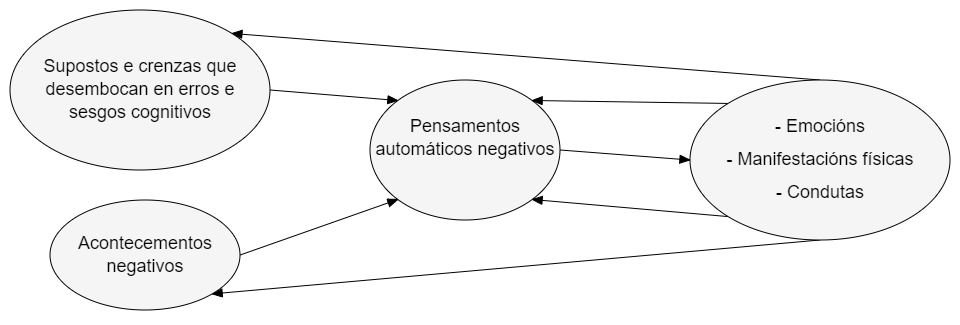
\includegraphics[width=0.46\linewidth]{tratamentos1_12_1}
	\caption{Modelo do desaxuste emocional e/ou condutual}
\end{figure}

\section{Tipos de cognicións}
\begin{itemize}
	\item \textbf{Pensamentos automáticos:} Imaxes e/ou autoverbalizacións que aparecen ante 
	estímulos internos e externos, como resultado da interacción entre supostos, crenzas, procesos 
	cognitivos e elementos situacionais. Algúns aspectos característicos deste tipo de pensamentos é 
	que surxen coma se foran reflexos, parecen totalmente plausibles e válidos e son involuntarios, 
	polo que costa detelos.
	\item \textbf{Supostos:} Crenzas condicionais, manifestadas a través de proposicións ``se ... 
	entón ...'', normas e actitudes. 
	\item \textbf{Crenzas nucleares:} Crenzas incondicionais, duradeiras e globais, sobre un mesmo, 
	os demais e o mundo. Son máis profundas e máis difíciles de modificar que os supostos, pero igual 
	ca estes, proveñen en gran medida de experiencias de aprendizaxe e relaciónanse en interacción co 
	medio. Tamén igual que os supostos, poden permanecer latentes e activarse debido a un 
	acontecemento importante, facendo que o suxeito cometa erros ou sesgos cognitivos.
\end{itemize}

\section{Fundamentos conceptuais e empíricos}
As distorsións ou erros cognitivos son erros sistemáticos no procesamento da información, isto é, no razoamento. Poden manifestarse de diferentes xeitos:
\begin{itemize}
	\item[$\diamond$] \underline{Inferencia arbitraria}: Conclusións negativas precipitadas, que o 
	paciente ten en forma de ``lector de mentes'' (supón o que os demais pensan) ou de ``erro do 
	adivino'' (espera que as cousas salan mal sen motivo).
	\item[$\diamond$] \underline{Xeralización excesiva}: Debido a un ou uns poucos sucesos negativos, 
	suponse que todos serán iguais.
	\item[$\diamond$] \underline{Filtro mental}: Centrarse nun único detalle negativo, obviando o 
	resto.
	\item[$\diamond$] \underline{Personalización}: Atribuirse toda a responsabilidade de sucesos que 
	teñen consecuencias negativas para os demais; comparación cos demais.
	\item[$\diamond$] \underline{Pensamento dicotómico}: Ver as situacións de forma extrema, sen ter 
	en conta a existencia de estados intermedios.
	\item[$\diamond$] \underline{Magnificación e minimización}: Esaxerar ou quitar, respectivamente, 
	a importancia que teñen as situacións.
	\item[$\diamond$] \underline{Descalificación do positivo}: Interpretar os propios comportamentos 
	positivos e os acontecementos agradables que ocoren como ``o normal''.
	\item[$\diamond$] \underline{Etiquetación}: Xeralizar unha (ou poucas) cualidade negativa para 
	dar lugar a un xuizo global.
	\item[$\diamond$] \underline{Os ``deberías''}: Esixencias absolutas e ríxidas, semellantes a 
	dogmas, acerca dun mesmo, dos demais e do mundo. 
\end{itemize}

\section{Procedemento en depresión}
A estrutura dunha sesión típica sería a seguinte:
\begin{enumerate}
	\item Breve revisión da sesión anterior e das actividades entre sesións (tarefas para casa).
	\item Fixación da orde do día e temas para a sesión. As prioridades determínanse conxuntamente, 
	dacordo coas preferencias do paciente.
	\item Novas tarefas para casa.
	\item Resumo da sesión e \textit{feedback}. 
\end{enumerate}

O procedemento da terapia desenvólvese en tres fases:
\begin{itemize}
	\item \textbf{Fase inicial:} Avaliación, conceptualización e xustificación da terapia.
	\begin{itemize}
		\item[1.] \underline{Relación terapéutica}: Entre as habilidades do terapeuta deben incluirse 
		o interese polo benestar do paciente, o coñecemento de si mesmo, a ética, a proximidade e o 
		coñecemento de contextos socio-culturais diversos. Entre as actitudes do terapeuta, son 
		importantes a calidez, a cordialidade, a autenticidade, a empatía e a aceptación positiva 
		incondicional.
		\item[2.] \underline{Avaliación do problema}: Ó longo da entrevista determinaranse os 
		síntomas anímicos, condutuais, cognitivos, psicofisiolóxicos e interpersoais. Para avaliar o 
		problema poden empregarse distintos métodos: preguntas directas, descubrimento guiado 
		(orientar o diálogo cara sucesos concretos que permitan determinar pensamentos, imaxes, 
		condutas...), momentos emocionais, inducción de estados emocionais, representacion de 
		interaccións, asignación e análise de tarefas condutuais e autorrexistros (de situacións, 
		emocións e pensamentos automáticos). 
		\item[3.] \underline{Modelo explicativo do problema e da terapia}: O paciente debe entender o 
		que lle pasa e por que. Tamén debe comprender o importante que é a súa participación para 
		solucionar o problema. Para explicar todo isto, pode ser útil o uso de exemplos. Por último, 
		debe explicárselle en que consiste a terapia e canto dura, a duración das sesións e a 
		periocidade das consultas. 
		\item[4.] \underline{Establecemento de obxectivos}: Específicos para cada caso, acórdanse co 
		paciente.
	\end{itemize}
	\item \textbf{Fase intermedia:} 
	\begin{itemize}
		\item[1.] \underline{Planificación de actividades (activación condutual)}: Consensuar co 
		paciente o que está disposto a intentar, e ser realista planificando as actividades. Comezar 
		por actividades sinxelas e moi gratificantes e ir aumentando a dificultade en función dos 
		resultados obtidos e da implicación do paciente.
		\item[2.] \underline{Identificación e cuestionamento de pensamentos automáticos}: Análise de 
		validez, de utilidade e doutros puntos de referencia, e reatribución (determinar que porción 
		de responsabilidade é atribuible ó paciente e cal a outros factores). Os pasos a seguir son:
		\begin{itemize}
			\item[a.] Identificar o problema.
			\item[b.] Identificar unha ou máis cognicións e avaliar o grao de crenza.
			\item[c.] Discutir o pensamento, instaurar un pensamento alternativo e avaliar o grao de 
			crenza.
			\item[d.] Facer unha predición específica que poida someterse a proba, e avaliar o grao 
			de crenza.
			\item[e.] Deseñar un experimento condutual para poñer a proba os pensamentos automáticos. 
			Estes experimentos consisten en emitir ou deixar de emitir unha conduta, observar a 
			reacción dos demais e preguntarlles acerca da situación.
			\item[f.] Avaliar o resultado, discutilo e extraer conclusións (avaliar o nivel de 
			crenza). 
		\end{itemize}
		\item[3.] \underline{Identificación e cuestionamento de supostos e crenzas}: As ideas 
		irracionais son crenzas centrais negativas, instauradas nun nivel profundo da conciencia, 
		formando parte dos valores fundamentais da persoa. Son ríxidas e pouco realistas, non se 
		apoian na experiencia. Adoitan incluir contidos acerca da persoa, dos demais e do mundo. 
		
		Para a identificación das crenzas poden empregarse varios métodos:
		\begin{itemize}
			\item \textbf{Inferencia de regras xerais:} Inferir ideas de fondo subxacentes a partir 
			de pensamentos concretos.
			\item \textbf{Contidos de regras e normas:} Explorar o significado oculto dos ``debería'' 
			e dos ``teño que''.
			\item \textbf{Análise de expresións:} Concretamente daquelas que o paciente poida 
			reiterar, coma se se tratase de refráns.
			\item \textbf{Uso de cuestionarios:} Por exemplo, o \textit{Dysfunctional Attitude Scale} 
			(Weissman e Beck, 1978).
			\item \textbf{Técnica da frecha descendente:} Consiste en realizar preguntas sucesivas 
			sobre as distintas afirmacións do paciente, para que el mesmo identifique as súas crenzas 
			irracionais.
			\item \textbf{Búsqueda de valores:} Indagar na xerarquía de valores do paciente para 
			atopar aqueles que poden resultar disfuncionais.
		\end{itemize}
		
		Á hora de cuestionar as crenzas, deben examinarse as probas a favor e en contra das mesmas, 
		analizar a súa utilidade e buscar e fortalecer crenzas alternativas. 
	\end{itemize}
	\item \textbf{Fase final. Prevención de recaídas:} Importante que o paciente domine as 
	habilidades aprendidas e as poña en práctica. Ante a posibilidade de que aparezan situacións 
	conflitivas, débense deseñar programas con técnicas para afrontalas. Realizar un seguimento do 
	paciente e non baixar a garda. 
\end{itemize}

\end{document}